\subsection{Analisis Kebutuhan Sistem}
\label{sec:analisis-kebutuhan-sistem}

Berdasarkan beberapa pendekatan yang telah dijelaskan pada \textbf{Bagian \ref{sec:analisis-solusi}}, Membuat sistem \textit{remote deployment}, yang dirancang untuk provisioning skala besar dari aplikasi pada perangkat \textit{IoT} yang terbatas sumber daya, menggunakan Kubernetes menjadi solusi yang digunakan karena beberapa keuntungan yang tidak dimiliki oleh pendekatan lain. Kubernetes, sebagai sistem orkestrasi kontainer yang matang dan luas digunakan, menawarkan fitur dan kemampuan yang cocok untuk mengatasi tantangan yang dihadapi dalam lingkungan \textit{IoT} yang heterogen dan terdistribusi terutama dalam masalah skalabilitas, \textit{ready to use}, serta memakan waktu yang minimal sehingga solusi ini merupakan solusi paling feasible yang dapat diimplementasikan. Sebelum sistem dibuat, langkah pertama yaitu membuat dan mencari kebutuhan sistem yang diperlukan. Kebutuhan sistem dibagi menjadi kebutuhan fungsional dan non-fungsional.

\subsubsection{Deskripsi sistem}
Sistem yang dibuat merupakan sebuah sistem yang dapat melakukan sebuah aksi, command, ataupun \textit{remote deployment} ke perangkat yang terhubung ataupun ke sebagian perangkat yang diinginkan. Sistem memiliki dua komponen utama yaitu dashboard sebagai \textit{frontend} serta API sebagai \textit{backend}. Komponen \textit{backend} ini memiliki dua modul eksternal dan satu modul internal. Kubernetes dan database sebagai modul eksternal serta server sebagai penghubung modul eksternal sebagai modul internal. Modul kubernetes terhubung ke kluster yang diinginkan untuk melakukan proses \textit{remote deployment} ke masing masing perangkat yang terhubung. Illustrasi secara kasar dapat dilihat pada gambar \ref{fig:gambaran-umum-arsitektur}

\begin{figure}[ht]
  \centering
  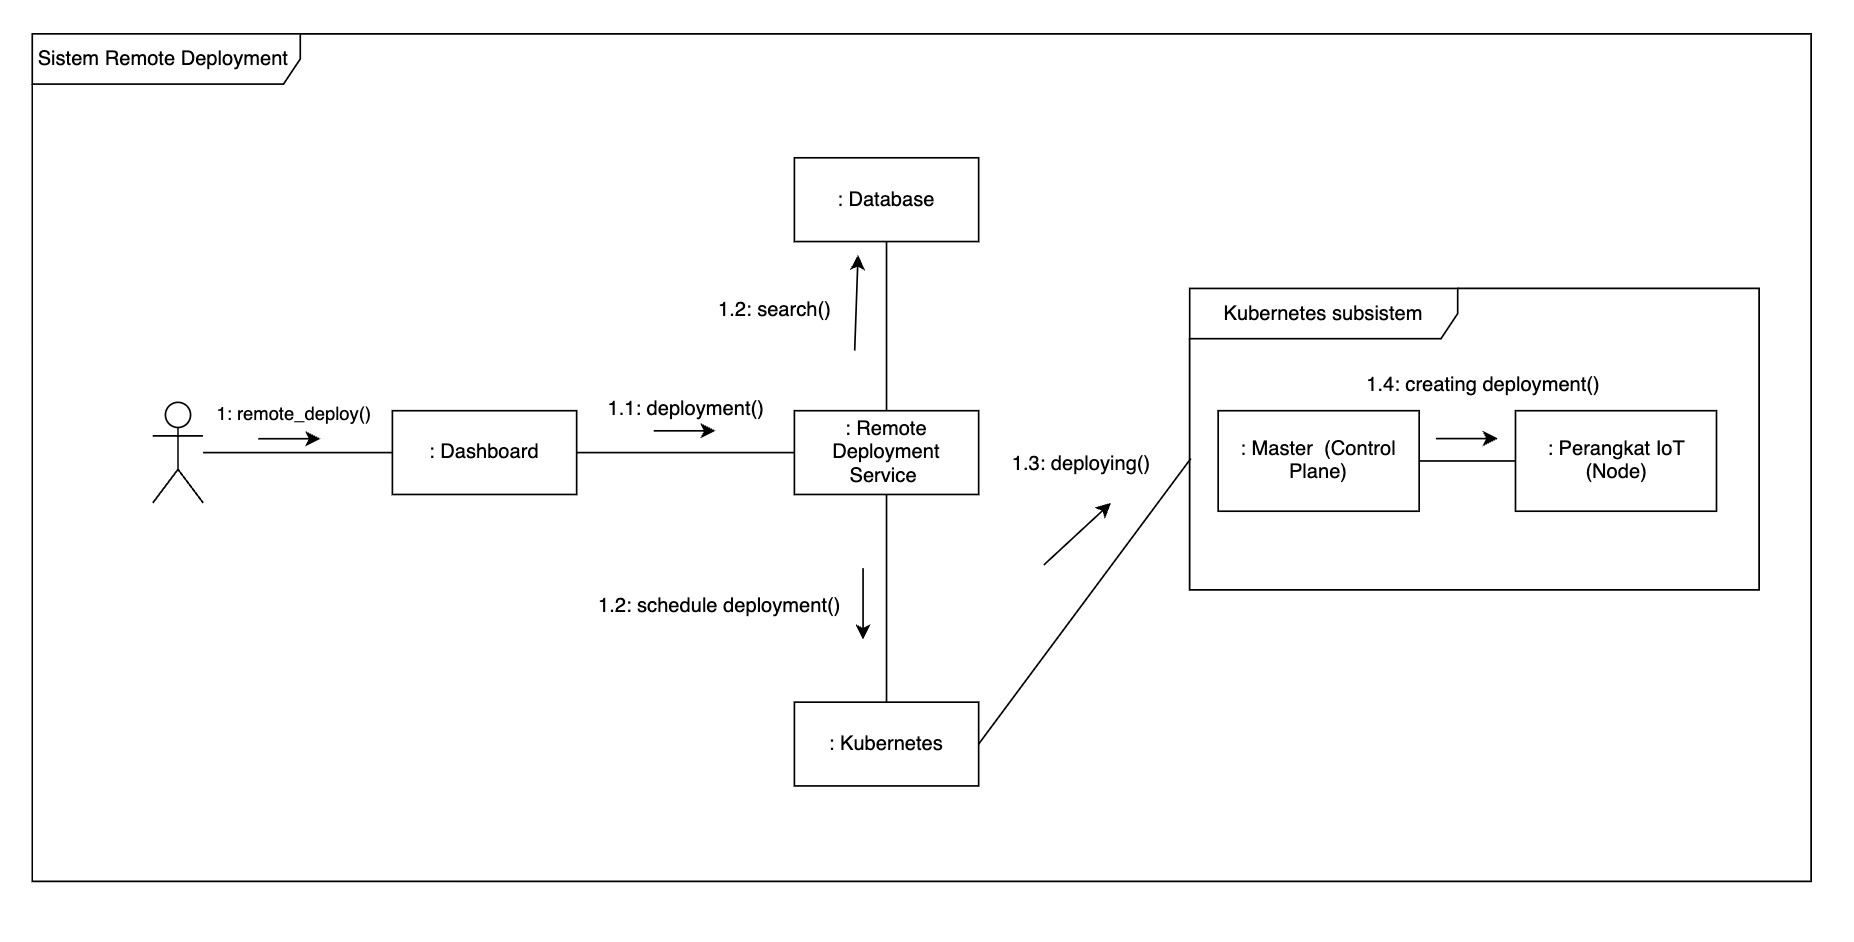
\includegraphics[width=1\textwidth]{resources/chapter-3/gambaran-umum-arsitektur-updated.jpg}
  \caption{Gambaran Umum Arsitektur}
  \label{fig:gambaran-umum-arsitektur}
\end{figure}

\pagebreak
\subsubsection{Karakteristik Pengguna}
Berdasarkan hasil analisis terdapat dua pengguna pada sistem ini. Yaitu pengguna dan administrator. Penjelasan lebih detil dapat dilihat pada tabel dibawah ini.


\begin{table}[h]
  \caption{Karakteristik Pengguna}
  \label{tab:karakteristik-pengguna}
  \centering
  \begin{tabular}{|p{2cm}|p{8cm}|}
    \hline
    Kategori Pengguna & Hak akses                                                                                                                                                                                                                                                                           \\
    \hline
    \textit{User}     & \textit{User} dapat melakukan login, registrasi, melihat \textit{user} lain di satu perusahaan, melakukan manajemen perangkat, melakukan manajemen groups, melakukan manajemen \textit{deployment}, melakukan \textit{remote deployment}, serta melihat riwayat \textit{deployment} \\
    \hline
    Admin             & Admin dapat melakukan manajemen perusahaan, manajemen user, serta seluruh kegiatan yang user dapat lakukan                                                                                                                                                                          \\
    \hline
  \end{tabular}
\end{table}

\subsubsection{Kebutuhan Fungsional}
Berikut merupakan kebutuhan fungsional dari sistem yang akan dibuat, agar lebih jelas kebutuhan fungsional dibuat ke dalam bentuk tabel di bawah ini. Semua kebutuhan fungsional akan memiliki ID yang diawali dengan huruf F lalu diikuti dengan dua angka.

\begin{table}
  \caption{Kebutuhan Fungsional}
  \label{tab:kebutuhan-fungsional}
  \centering
  \begin{tabular}{|c|p{4.5cm}|p{8cm}|}
    \hline
    ID  & Kebutuhan                                                                      & Penjelasan                                                                                                 \\
    \hline
    F01 & Sistem dapat meregistrasi perusahaan                                           & Admin dapat melakukan registrasi perusahaan baru ke dalam database sistem.                                 \\
    \hline
    F02 & Sistem dapat melihat seluruh perusahaan yang terdaftar                         & Admin dapat melihat seluruh perushaan yang ada pada database sistem.                                       \\
    \hline
    F03 & Sistem dapat melihat detail perusahaan                                         & Pengguna dapat melihat detail dari perushaan yang ada pada database sistem.                                \\
    \hline
    F04 & Sistem dapat melihat seluruh pengguna pada suatu perusahaan                    & Pengguna dapat melihat pengguna lain pada satu perusahaan yang sama                                        \\
    \hline
    F05 & Sistem dapat meregistrasi pengguna                                             & Admin dapat melakukan registrasi pengguna baru ke sebuah perusahaan pada sistem.                           \\
    \hline
    F06 & Sistem dapat menghapus pengguna                                                & Admin dapat menghapus pengguna dari suatu perusahaan                                                       \\
    \hline
    F07 & Sistem dapat melakukan authentikasi pengguna                                   & Pengguna dapat masuk ke dalam sistem dengan memasukan kredensial yang diberikan.                           \\
    \hline
    F08 & Sistem dapat menghapus authentikasi pengguna                                   & Pengguna dapat \textit{logout} dari sistem.                                                                \\
    \hline
    F09 & Sistem dapat meregistrasi perangkat \textit{IoT}                               & Pengguna dapat melakukan registrasi perangkat ke database sistem                                           \\
    \hline
    F10 & Sistem dapat melihat perangkat yang terdaftar                                  & Pengguna dapat melihat seluruh perangkat yang telah didaftarkan pada perushaannya                          \\
    \hline
    F11 & Sistem dapat menghapus perangkat yang terdaftar                                & Pengguna dapat menghapus perangkat yang telah didaftarkan di database                                      \\
    \hline
    F12 & Sistem dapat membuat \textit{groups}                                           & Pengguna dapat membuat \textit{groups} untuk mengelompokan beberapa perangkat                              \\
    \hline
    F13 & Sistem dapat melihat seluruh \textit{groups} yang telah didaftarkan            & Pengguna dapat melihat seluruh \textit{groups} yang telah terdaftar pada perusahannya                      \\
    \hline
    F14 & Sistem dapat menghapus \textit{groups} yang telah didaftarkan                  & Pengguna dapat menghapus \textit{groups} yang telah terdaftar pada perusahannya                            \\
    \hline
    F15 & Sistem dapat melihat seluruh perangkat yang terasosiasi dengan \textit{groups} & Pengguna dapat melihat hubungan antara perangkat dan \textit{groups} pada sistem dan begitupula sebaliknya \\
    \hline
    F16 & Sistem dapat membuat deployment images                                         & Pengguna dapat membuat deployment images yang teraosiasi dengan perusahannya                               \\
    \hline
    F17 & Sistem dapat melihat deployment images yang terdaftar                          & Pengguna dapat melihat deployment images yang teraosiasi dengan perusahannya                               \\
    \hline
  \end{tabular}
\end{table}

\begin{table}
  \centering
  \begin{tabular}{|c|p{4.5cm}|p{8cm}|}
    \hline
    ID  & Kebutuhan                                               & Penjelasan                                                                                       \\
    \hline
    F18 & Sistem dapat menghapus deployment images yang terdaftar & Pengguna dapat menghapus deployment images yang teraosiasi dengan perusahannya                   \\
    \hline
    F19 & Sistem dapat membuat deployment plan                    & Pengguna dapat membuat deployment plan yang teraosiasi dengan perushaannya                       \\
    \hline
    F20 & Sistem dapat melihat deployment plan yang terdaftar     & Pengguna dapat melihat seluruh deployment plan yang terdaftar dan teraosiasi dengan perushaannya \\
    \hline
    F21 & Sistem dapat menghapus deployment plan yang terdaftar   & Pengguna dapat menghapus deployment plan yang terdaftar dan teraosiasi dengan perushaannya       \\
    \hline
    F22 & Sistem dapat melihat melakukan deployment               & pengguna dapat melakukan deployment ke perangkat ataupun group dengan deployment plan pilihannya \\
    \hline
    F23 & Sistem dapat melihat  deployment history                & pengguna dapat melihat riwayat dari deployment yang telah dilakukan ke perangkat ataupun group   \\
    \hline
  \end{tabular}
\end{table}

\pagebreak

Relasi antara aktor yang telah didefinisikan dengan kapabilitas fungsional sistem dapat dilihat pada diagram use case berikut.

\begin{figure}[h]
  \centering
  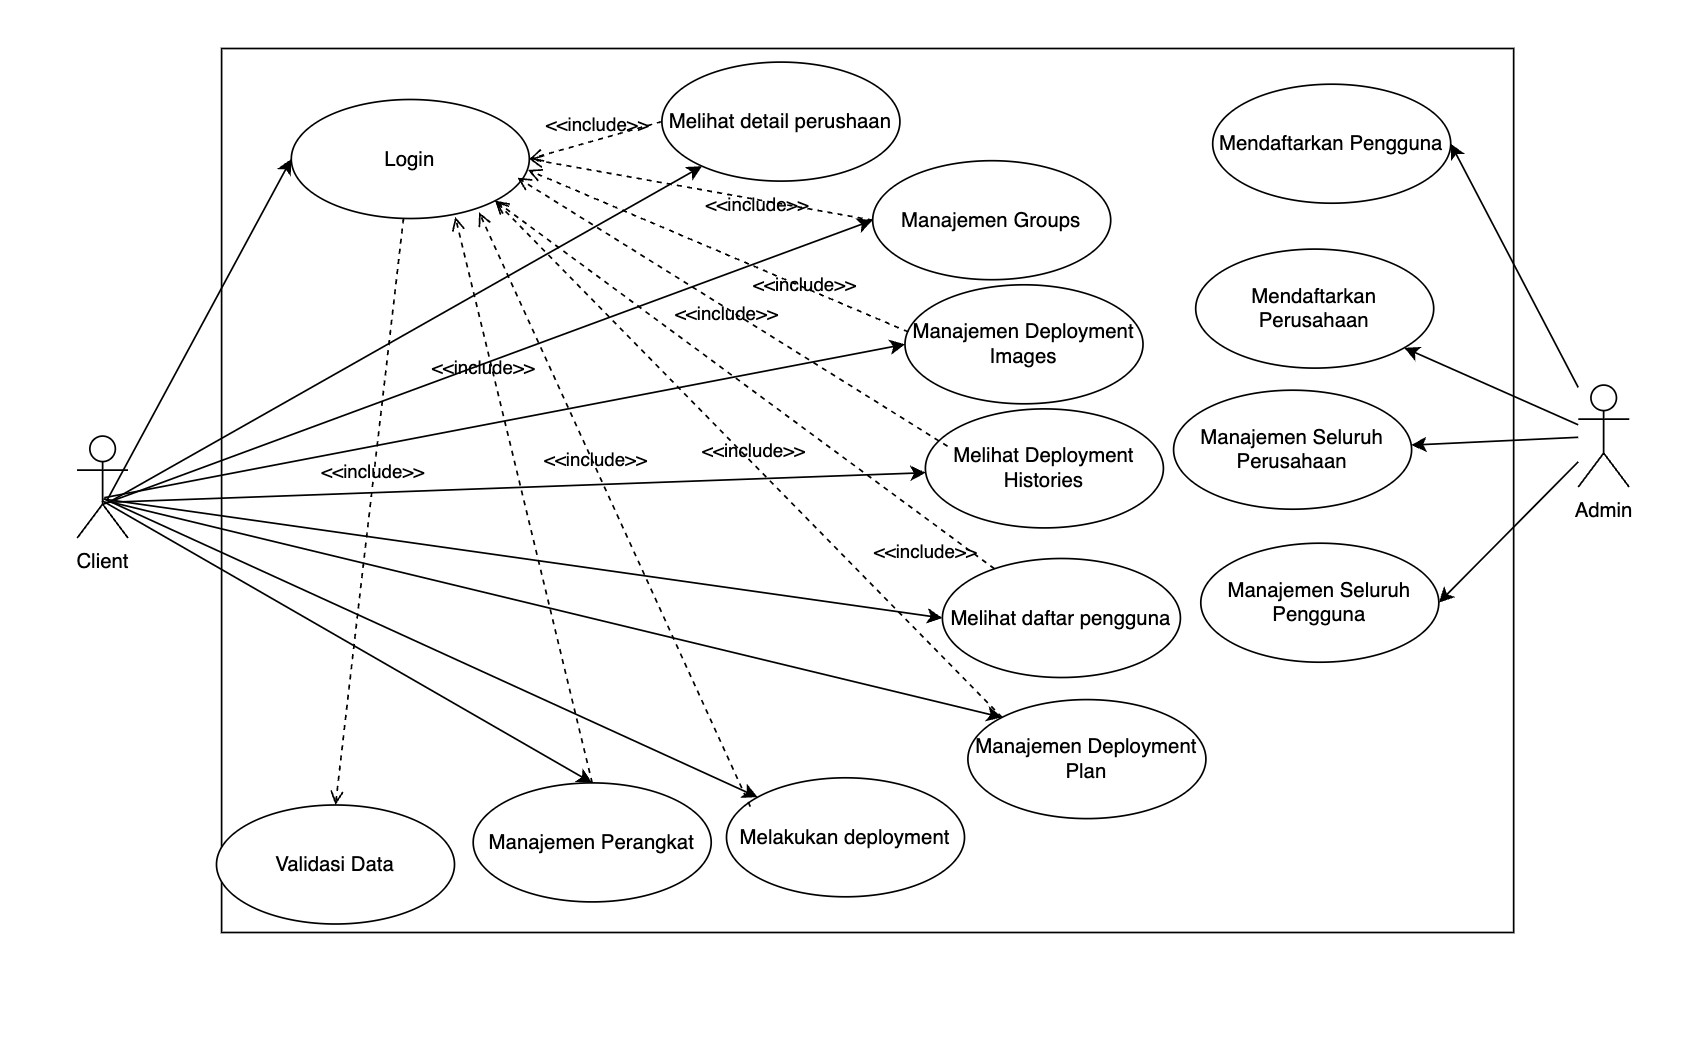
\includegraphics[width=1\textwidth]{resources/chapter-3/usecase-diagram.jpg}
  \caption{Usecase Diagram}
  \label{fig:usecase-diagram}
\end{figure}

\subsubsection{Kebutuhan Non-Fungsional}
Berikut merupakan kebutuhan non fungsional dari sistem yang akan dibuat, agar lebih jelas kebutuhan non fungsional dibuat ke dalam bentuk tabel. Semua kebutuhan non-fungsional memiliki awalan ID NF lalu diikuti oleh dua angka. Terdapat lima parameter non fungsional yang dapat dilihat pada tabel di bawah ini.
\begin{table}[ht]
  \caption{Kebutuhan Non-Fungsional}
  \label{tab:kebutuhan-non-fungsional}
  \centering
  \begin{tabular}{|c|p{3cm}|p{8cm}|}
    \hline
    ID   & Parameter      & Kebutuhan                                                  \\
    \hline
    NF01 & Availability   & Tingkat ketersediaan sistem minimal 98\%                   \\
    \hline
    NF02 & Maintanability & Sistem dapat dimaintain dari jauh dengan mudah             \\
    \hline
    NF03 & Security       & Sistem akan menjamin keamanan dari masing masing perangkat \\
    \hline
    NF04 & Safety         & Sistem akan menjamin keamanan dari masing masing perangkat \\
    \hline
    NF05 & Portability    & Sistem dapat diakses dimana saja menggunakan komputer      \\
    \hline
  \end{tabular}
\end{table}

\subsubsection{Model \textit{Use case}}
\label{subsec:model-usecase}
Dari beberapa kebutuhan fungsional serta karakteristik pengguna, dapat dibuat \textit{use case} yang mengelompokan serta menggambarkan relasi antara aktor dan aksi yang dapat dilakukan. Use case akan memiliki identifikasi yang berawalan dengan UC diikuti oleh dua angka. Use case dapat dilihat secara detail pada tabel \ref{tab:penjelasan-usecase-diagram}

Dari pemetaan \textit{Use case} pada tabel \ref{tab:penjelasan-usecase-diagram}, dapat dibuat sebuah diagram yang menghubungkan relasi antara aktor dengan usecasenya. Relasi  aktor dengan kapabilitas fungsional sistem dapat dilihat pada diagram use case berikut.

\begin{figure}[ht]
  \centering
  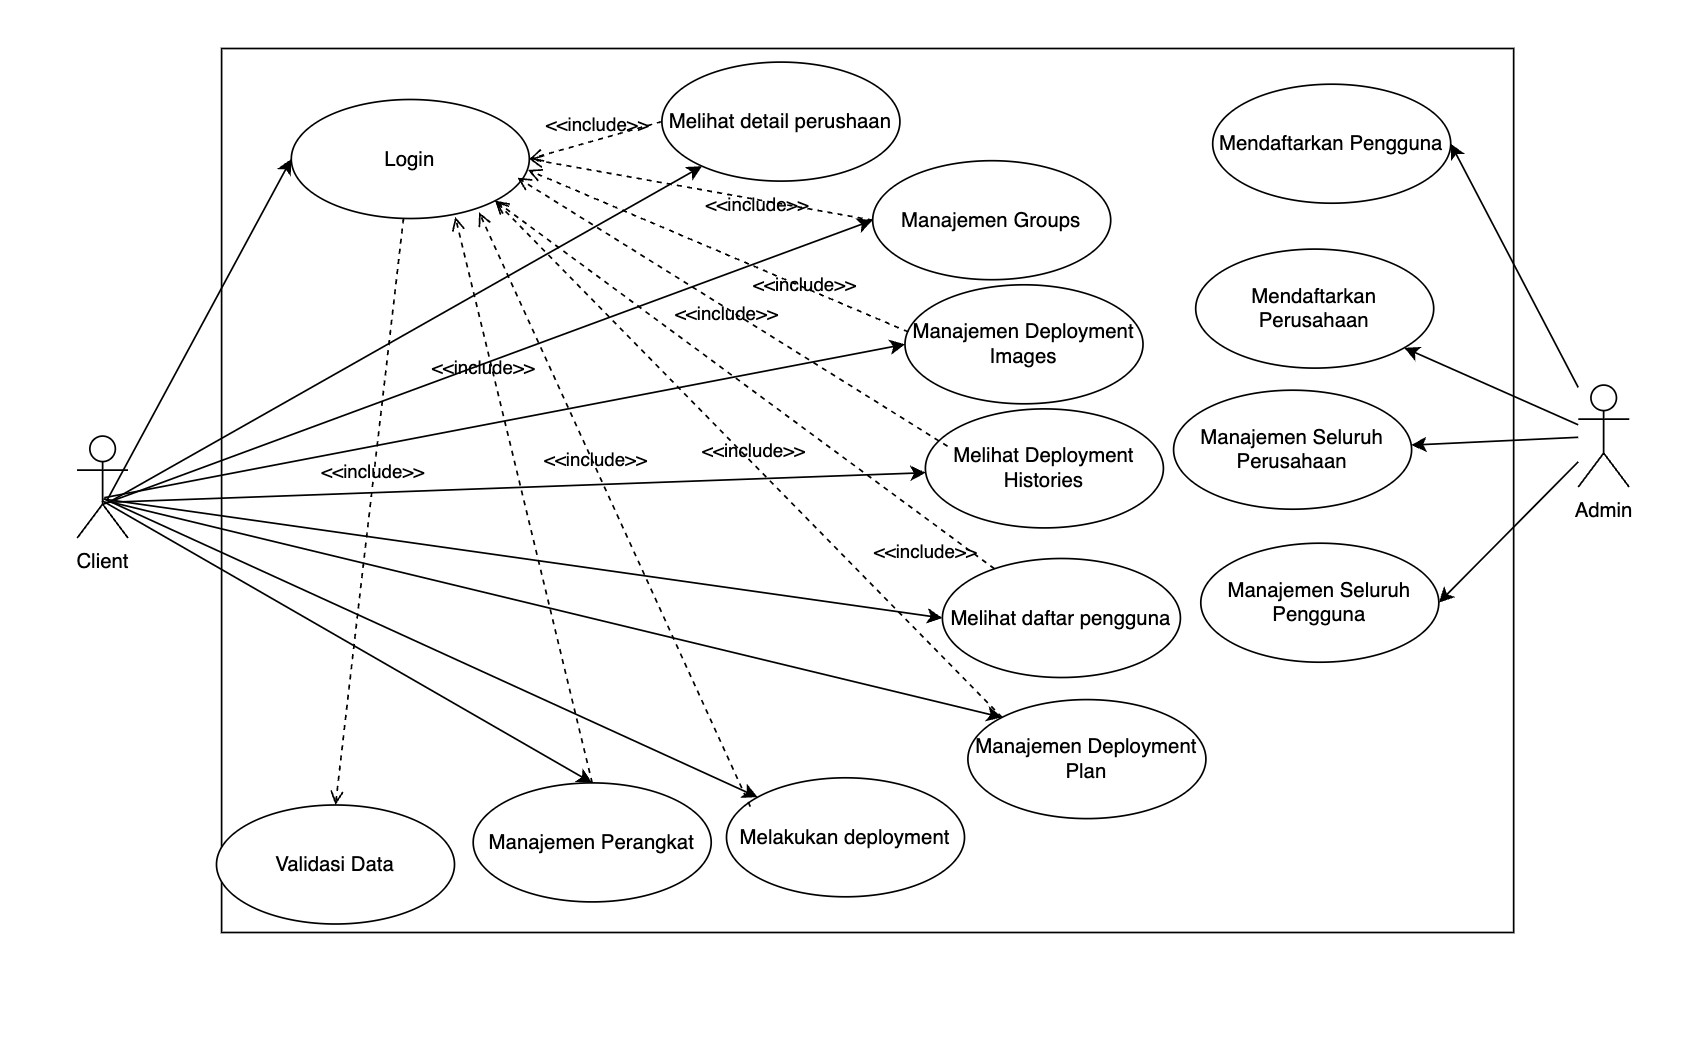
\includegraphics[width=1\textwidth]{resources/chapter-3/usecase-diagram.jpg}
  \caption{Usecase Diagram}
  \label{fig:usecase-diagram}
\end{figure}
